\documentclass[1p]{elsarticle_modified}
%\bibliographystyle{elsarticle-num}

%\usepackage[colorlinks]{hyperref}
%\usepackage{abbrmath_seonhwa} %\Abb, \Ascr, \Acal ,\Abf, \Afrak
\usepackage{amsfonts}
\usepackage{amssymb}
\usepackage{amsmath}
\usepackage{amsthm}
\usepackage{scalefnt}
\usepackage{amsbsy}
\usepackage{kotex}
\usepackage{caption}
\usepackage{subfig}
\usepackage{color}
\usepackage{graphicx}
\usepackage{xcolor} %% white, black, red, green, blue, cyan, magenta, yellow
\usepackage{float}
\usepackage{setspace}
\usepackage{hyperref}

\usepackage{tikz}
\usetikzlibrary{arrows}

\usepackage{multirow}
\usepackage{array} % fixed length table
\usepackage{hhline}

%%%%%%%%%%%%%%%%%%%%%
\makeatletter
\renewcommand*\env@matrix[1][\arraystretch]{%
	\edef\arraystretch{#1}%
	\hskip -\arraycolsep
	\let\@ifnextchar\new@ifnextchar
	\array{*\c@MaxMatrixCols c}}
\makeatother %https://tex.stackexchange.com/questions/14071/how-can-i-increase-the-line-spacing-in-a-matrix
%%%%%%%%%%%%%%%

\usepackage[normalem]{ulem}

\newcommand{\msout}[1]{\ifmmode\text{\sout{\ensuremath{#1}}}\else\sout{#1}\fi}
%SOURCE: \msout is \stkout macro in https://tex.stackexchange.com/questions/20609/strikeout-in-math-mode

\newcommand{\cancel}[1]{
	\ifmmode
	{\color{red}\msout{#1}}
	\else
	{\color{red}\sout{#1}}
	\fi
}

\newcommand{\add}[1]{
	{\color{blue}\uwave{#1}}
}

\newcommand{\replace}[2]{
	\ifmmode
	{\color{red}\msout{#1}}{\color{blue}\uwave{#2}}
	\else
	{\color{red}\sout{#1}}{\color{blue}\uwave{#2}}
	\fi
}

\newcommand{\Sol}{\mathcal{S}} %segment
\newcommand{\D}{D} %diagram
\newcommand{\A}{\mathcal{A}} %arc


%%%%%%%%%%%%%%%%%%%%%%%%%%%%%5 test

\def\sl{\operatorname{\textup{SL}}(2,\Cbb)}
\def\psl{\operatorname{\textup{PSL}}(2,\Cbb)}
\def\quan{\mkern 1mu \triangleright \mkern 1mu}

\theoremstyle{definition}
\newtheorem{thm}{Theorem}[section]
\newtheorem{prop}[thm]{Proposition}
\newtheorem{lem}[thm]{Lemma}
\newtheorem{ques}[thm]{Question}
\newtheorem{cor}[thm]{Corollary}
\newtheorem{defn}[thm]{Definition}
\newtheorem{exam}[thm]{Example}
\newtheorem{rmk}[thm]{Remark}
\newtheorem{alg}[thm]{Algorithm}

\newcommand{\I}{\sqrt{-1}}
\begin{document}

%\begin{frontmatter}
%
%\title{Boundary parabolic representations of knots up to 8 crossings}
%
%%% Group authors per affiliation:
%\author{Yunhi Cho} 
%\address{Department of Mathematics, University of Seoul, Seoul, Korea}
%\ead{yhcho@uos.ac.kr}
%
%
%\author{Seonhwa Kim} %\fnref{s_kim}}
%\address{Center for Geometry and Physics, Institute for Basic Science, Pohang, 37673, Korea}
%\ead{ryeona17@ibs.re.kr}
%
%\author{Hyuk Kim}
%\address{Department of Mathematical Sciences, Seoul National University, Seoul 08826, Korea}
%\ead{hyukkim@snu.ac.kr}
%
%\author{Seokbeom Yoon}
%\address{Department of Mathematical Sciences, Seoul National University, Seoul, 08826,  Korea}
%\ead{sbyoon15@snu.ac.kr}
%
%\begin{abstract}
%We find all boundary parabolic representation of knots up to 8 crossings.
%
%\end{abstract}
%\begin{keyword}
%    \MSC[2010] 57M25 
%\end{keyword}
%
%\end{frontmatter}

%\linenumbers
%\tableofcontents
%
\newcommand\colored[1]{\textcolor{white}{\rule[-0.35ex]{0.8em}{1.4ex}}\kern-0.8em\color{red} #1}%
%\newcommand\colored[1]{\textcolor{white}{ #1}\kern-2.17ex	\textcolor{white}{ #1}\kern-1.81ex	\textcolor{white}{ #1}\kern-2.15ex\color{red}#1	}

{\Large $\underline{9_{27}~(K9a_{12})}$}

\setlength{\tabcolsep}{10pt}
\renewcommand{\arraystretch}{1.6}
\vspace{1cm}\begin{tabular}{m{100pt}>{\centering\arraybackslash}m{274pt}}
\multirow{5}{120pt}{
	\centering
	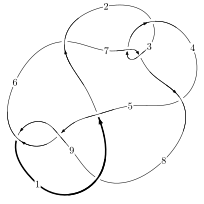
\includegraphics[width=112pt]{../../../GIT/diagram.site/Diagrams/png/62_9_27.png}\\
\ \ \ A knot diagram\footnotemark}&
\allowdisplaybreaks
\textbf{Linearized knot diagam} \\
\cline{2-2}
 &
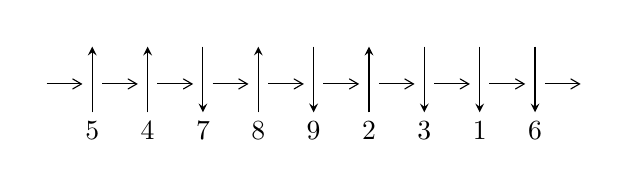
\begin{tikzpicture}[x=20pt, y=17pt]
	% nodes
	\node (C0) at (0, 0) {};
	\node (C1) at (1, 0) {};
	\node (C1U) at (1, +1) {};
	\node (C1D) at (1, -1) {5};

	\node (C2) at (2, 0) {};
	\node (C2U) at (2, +1) {};
	\node (C2D) at (2, -1) {4};

	\node (C3) at (3, 0) {};
	\node (C3U) at (3, +1) {};
	\node (C3D) at (3, -1) {7};

	\node (C4) at (4, 0) {};
	\node (C4U) at (4, +1) {};
	\node (C4D) at (4, -1) {8};

	\node (C5) at (5, 0) {};
	\node (C5U) at (5, +1) {};
	\node (C5D) at (5, -1) {9};

	\node (C6) at (6, 0) {};
	\node (C6U) at (6, +1) {};
	\node (C6D) at (6, -1) {2};

	\node (C7) at (7, 0) {};
	\node (C7U) at (7, +1) {};
	\node (C7D) at (7, -1) {3};

	\node (C8) at (8, 0) {};
	\node (C8U) at (8, +1) {};
	\node (C8D) at (8, -1) {1};

	\node (C9) at (9, 0) {};
	\node (C9U) at (9, +1) {};
	\node (C9D) at (9, -1) {6};
	\node (C10) at (10, 0) {};

	% arrows
	\draw[->,>={angle 60}]
	(C0) edge (C1) (C1) edge (C2) (C2) edge (C3) (C3) edge (C4) (C4) edge (C5) (C5) edge (C6) (C6) edge (C7) (C7) edge (C8) (C8) edge (C9) (C9) edge (C10) ;	\draw[->,>=stealth]
	(C1D) edge (C1U) (C2D) edge (C2U) (C3U) edge (C3D) (C4D) edge (C4U) (C5U) edge (C5D) (C6D) edge (C6U) (C7U) edge (C7D) (C8U) edge (C8D) (C9U) edge (C9D) ;
	\end{tikzpicture} \\
\hhline{~~} \\& 
\textbf{Solving Sequence} \\ \cline{2-2} 
 &
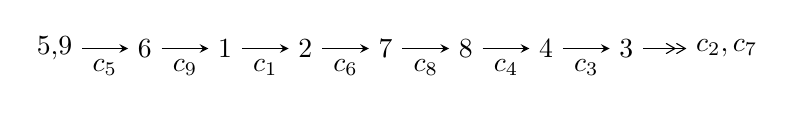
\begin{tikzpicture}[x=29pt, y=7pt]
	% node
	\node (A0) at (-1/8, 0) {5,9};
	\node (A1) at (1, 0) {6};
	\node (A2) at (2, 0) {1};
	\node (A3) at (3, 0) {2};
	\node (A4) at (4, 0) {7};
	\node (A5) at (5, 0) {8};
	\node (A6) at (6, 0) {4};
	\node (A7) at (7, 0) {3};
	\node (C1) at (1/2, -1) {$c_{5}$};
	\node (C2) at (3/2, -1) {$c_{9}$};
	\node (C3) at (5/2, -1) {$c_{1}$};
	\node (C4) at (7/2, -1) {$c_{6}$};
	\node (C5) at (9/2, -1) {$c_{8}$};
	\node (C6) at (11/2, -1) {$c_{4}$};
	\node (C7) at (13/2, -1) {$c_{3}$};
	\node (A8) at (33/4, 0) {$c_{2},c_{7}$};

	% edge
	\draw[->,>=stealth]	
	(A0) edge (A1) (A1) edge (A2) (A2) edge (A3) (A3) edge (A4) (A4) edge (A5) (A5) edge (A6) (A6) edge (A7) ;
	\draw[->>,>={angle 60}]	
	(A7) edge (A8);
\end{tikzpicture} \\ 

\end{tabular} \\

\footnotetext{
The image of knot diagram is generated by the software ``\textbf{Draw programme}" developed by Andrew Bartholomew(\url{http://www.layer8.co.uk/maths/draw/index.htm\#Running-draw}), where we modified some parts for our purpose(\url{https://github.com/CATsTAILs/LinksPainter}).
}\phantom \\ \newline 
\centering \textbf{Ideals for irreducible components\footnotemark of $X_{\text{par}}$} 
 
\begin{align*}
I^u_{1}&=\langle 
u^{24}+u^{23}+\cdots+2 u^3+1\rangle \\
\\
\end{align*}
\raggedright * 1 irreducible components of $\dim_{\mathbb{C}}=0$, with total 24 representations.\\
\footnotetext{All coefficients of polynomials are rational numbers. But the coefficients are sometimes approximated in decimal forms when there is not enough margin.}
\newpage
\renewcommand{\arraystretch}{1}
\centering \section*{I. $I^u_{1}= \langle u^{24}+u^{23}-5 u^{22}-6 u^{21}+13 u^{20}+18 u^{19}-20 u^{18}-34 u^{17}+19 u^{16}+44 u^{15}-10 u^{14}-42 u^{13}+2 u^{12}+32 u^{11}-22 u^9+13 u^7+u^6-6 u^5- u^4+2 u^3+1 \rangle$}
\flushleft \textbf{(i) Arc colorings}\\
\begin{tabular}{m{7pt} m{180pt} m{7pt} m{180pt} }
\flushright $a_{5}=$&$\begin{pmatrix}1\\0\end{pmatrix}$ \\
\flushright $a_{9}=$&$\begin{pmatrix}0\\u\end{pmatrix}$ \\
\flushright $a_{6}=$&$\begin{pmatrix}1\\u^2\end{pmatrix}$ \\
\flushright $a_{1}=$&$\begin{pmatrix}- u\\- u^3+u\end{pmatrix}$ \\
\flushright $a_{2}=$&$\begin{pmatrix}- u^3\\- u^3+u\end{pmatrix}$ \\
\flushright $a_{7}=$&$\begin{pmatrix}u^8- u^6+u^4+1\\u^8-2 u^6+2 u^4\end{pmatrix}$ \\
\flushright $a_{8}=$&$\begin{pmatrix}u^3\\u^5- u^3+u\end{pmatrix}$ \\
\flushright $a_{4}=$&$\begin{pmatrix}u^8- u^6+u^4+1\\u^{10}-2 u^8+3 u^6-2 u^4+u^2\end{pmatrix}$ \\
\flushright $a_{3}=$&$\begin{pmatrix}u^{21}-4 u^{19}+9 u^{17}-12 u^{15}+12 u^{13}-10 u^{11}+9 u^9-6 u^7+3 u^5-2 u^3+u\\u^{23}-5 u^{21}+\cdots-3 u^5+u\end{pmatrix}$\\ \flushright $a_{3}=$&$\begin{pmatrix}u^{21}-4 u^{19}+9 u^{17}-12 u^{15}+12 u^{13}-10 u^{11}+9 u^9-6 u^7+3 u^5-2 u^3+u\\u^{23}-5 u^{21}+\cdots-3 u^5+u\end{pmatrix}$\\&\end{tabular}
\flushleft \textbf{(ii) Obstruction class $= -1$}\\~\\
\flushleft \textbf{(iii) Cusp Shapes $= -4 u^{23}+24 u^{21}+4 u^{20}-72 u^{19}-20 u^{18}+132 u^{17}+52 u^{16}-160 u^{15}-84 u^{14}+132 u^{13}+92 u^{12}-84 u^{11}-72 u^{10}+52 u^9+44 u^8-32 u^7-24 u^6+8 u^5+12 u^4+4 u^3-4 u^2-2$}\\~\\
\newpage\renewcommand{\arraystretch}{1}
\flushleft \textbf{(iv) u-Polynomials at the component}\newline \\
\begin{tabular}{m{50pt}|m{274pt}}
Crossings & \hspace{64pt}u-Polynomials at each crossing \\
\hline $$\begin{aligned}c_{1}\end{aligned}$$&$\begin{aligned}
&u^{24}+3 u^{23}+\cdots+4 u+1
\end{aligned}$\\
\hline $$\begin{aligned}c_{2}\end{aligned}$$&$\begin{aligned}
&u^{24}-13 u^{23}+\cdots-2 u^2+1
\end{aligned}$\\
\hline $$\begin{aligned}c_{3},c_{7}\end{aligned}$$&$\begin{aligned}
&u^{24}+u^{23}+\cdots+2 u+1
\end{aligned}$\\
\hline $$\begin{aligned}c_{4},c_{6}\end{aligned}$$&$\begin{aligned}
&u^{24}- u^{23}+\cdots-10 u+1
\end{aligned}$\\
\hline $$\begin{aligned}c_{5},c_{9}\end{aligned}$$&$\begin{aligned}
&u^{24}+u^{23}+\cdots+2 u^3+1
\end{aligned}$\\
\hline $$\begin{aligned}c_{8}\end{aligned}$$&$\begin{aligned}
&u^{24}+11 u^{23}+\cdots-2 u^2+1
\end{aligned}$\\
\hline
\end{tabular}\\~\\
\newpage\renewcommand{\arraystretch}{1}
\flushleft \textbf{(v) Riley Polynomials at the component}\newline \\
\begin{tabular}{m{50pt}|m{274pt}}
Crossings & \hspace{64pt}Riley Polynomials at each crossing \\
\hline $$\begin{aligned}c_{1}\end{aligned}$$&$\begin{aligned}
&y^{24}+y^{23}+\cdots+20 y+1
\end{aligned}$\\
\hline $$\begin{aligned}c_{2}\end{aligned}$$&$\begin{aligned}
&y^{24}-3 y^{23}+\cdots-4 y+1
\end{aligned}$\\
\hline $$\begin{aligned}c_{3},c_{7}\end{aligned}$$&$\begin{aligned}
&y^{24}+13 y^{23}+\cdots-2 y^2+1
\end{aligned}$\\
\hline $$\begin{aligned}c_{4},c_{6}\end{aligned}$$&$\begin{aligned}
&y^{24}-19 y^{23}+\cdots-48 y+1
\end{aligned}$\\
\hline $$\begin{aligned}c_{5},c_{9}\end{aligned}$$&$\begin{aligned}
&y^{24}-11 y^{23}+\cdots-2 y^2+1
\end{aligned}$\\
\hline $$\begin{aligned}c_{8}\end{aligned}$$&$\begin{aligned}
&y^{24}+5 y^{23}+\cdots-4 y+1
\end{aligned}$\\
\hline
\end{tabular}\\~\\
\newpage\flushleft \textbf{(vi) Complex Volumes and Cusp Shapes}
$$\begin{array}{c|c|c}  
\text{Solutions to }I^u_{1}& \I (\text{vol} + \sqrt{-1}CS) & \text{Cusp shape}\\
 \hline 
\begin{aligned}
u &= -0.981563 + 0.214317 I\end{aligned}
 & -1.74298 + 0.40841 I & -5.87200 - 0.75563 I \\ \hline\begin{aligned}
u &= -0.981563 - 0.214317 I\end{aligned}
 & -1.74298 - 0.40841 I & -5.87200 + 0.75563 I \\ \hline\begin{aligned}
u &= \phantom{-}0.803335 + 0.491088 I\end{aligned}
 & \phantom{-}1.74384 - 2.05721 I & \phantom{-}4.27298 + 4.01793 I \\ \hline\begin{aligned}
u &= \phantom{-}0.803335 - 0.491088 I\end{aligned}
 & \phantom{-}1.74384 + 2.05721 I & \phantom{-}4.27298 - 4.01793 I \\ \hline\begin{aligned}
u &= -0.527198 + 0.744803 I\end{aligned}
 & \phantom{-}6.35994 + 2.92383 I & \phantom{-}5.29020 - 3.29300 I \\ \hline\begin{aligned}
u &= -0.527198 - 0.744803 I\end{aligned}
 & \phantom{-}6.35994 - 2.92383 I & \phantom{-}5.29020 + 3.29300 I \\ \hline\begin{aligned}
u &= \phantom{-}1.085860 + 0.107562 I\end{aligned}
 & \phantom{-}0.74814 + 3.77265 I & -1.89193 - 3.49106 I \\ \hline\begin{aligned}
u &= \phantom{-}1.085860 - 0.107562 I\end{aligned}
 & \phantom{-}0.74814 - 3.77265 I & -1.89193 + 3.49106 I \\ \hline\begin{aligned}
u &= -0.433290 + 0.779547 I\end{aligned}
 & \phantom{-}5.84506 - 5.78082 I & \phantom{-}4.37527 + 3.72629 I \\ \hline\begin{aligned}
u &= -0.433290 - 0.779547 I\end{aligned}
 & \phantom{-}5.84506 + 5.78082 I & \phantom{-}4.37527 - 3.72629 I \\ \hline\begin{aligned}
u &= -1.062920 + 0.387157 I\end{aligned}
 & -2.96425 + 1.34320 I & -6.02964 - 0.62000 I \\ \hline\begin{aligned}
u &= -1.062920 - 0.387157 I\end{aligned}
 & -2.96425 - 1.34320 I & -6.02964 + 0.62000 I \\ \hline\begin{aligned}
u &= \phantom{-}0.452781 + 0.717874 I\end{aligned}
 & \phantom{-}2.63437 + 1.18290 I & \phantom{-}1.39246 - 0.39910 I \\ \hline\begin{aligned}
u &= \phantom{-}0.452781 - 0.717874 I\end{aligned}
 & \phantom{-}2.63437 - 1.18290 I & \phantom{-}1.39246 + 0.39910 I \\ \hline\begin{aligned}
u &= \phantom{-}1.083310 + 0.462291 I\end{aligned}
 & -2.43992 - 5.71321 I & -4.10823 + 7.50361 I \\ \hline\begin{aligned}
u &= \phantom{-}1.083310 - 0.462291 I\end{aligned}
 & -2.43992 + 5.71321 I & -4.10823 - 7.50361 I \\ \hline\begin{aligned}
u &= -1.041780 + 0.614710 I\end{aligned}
 & \phantom{-}4.82981 + 2.24524 I & \phantom{-}3.02697 - 1.89383 I \\ \hline\begin{aligned}
u &= -1.041780 - 0.614710 I\end{aligned}
 & \phantom{-}4.82981 - 2.24524 I & \phantom{-}3.02697 + 1.89383 I \\ \hline\begin{aligned}
u &= \phantom{-}1.075010 + 0.585259 I\end{aligned}
 & \phantom{-}0.79700 - 6.17959 I & -1.78521 + 5.04555 I \\ \hline\begin{aligned}
u &= \phantom{-}1.075010 - 0.585259 I\end{aligned}
 & \phantom{-}0.79700 + 6.17959 I & -1.78521 - 5.04555 I \\ \hline\begin{aligned}
u &= -1.097340 + 0.604979 I\end{aligned}
 & \phantom{-}3.87224 + 11.00000 I & \phantom{-}1.31825 - 8.05284 I \\ \hline\begin{aligned}
u &= -1.097340 - 0.604979 I\end{aligned}
 & \phantom{-}3.87224 - 11.00000 I & \phantom{-}1.31825 + 8.05284 I \\ \hline\begin{aligned}
u &= \phantom{-}0.143789 + 0.548880 I\end{aligned}
 & \phantom{-}0.05596 + 1.77225 I & \phantom{-}0.01088 - 4.04184 I \\ \hline\begin{aligned}
u &= \phantom{-}0.143789 - 0.548880 I\end{aligned}
 & \phantom{-}0.05596 - 1.77225 I & \phantom{-}0.01088 + 4.04184 I\\
 \hline 
 \end{array}$$\newpage
\newpage\renewcommand{\arraystretch}{1}
\centering \section*{ II. u-Polynomials}
\begin{tabular}{m{50pt}|m{274pt}}
Crossings & \hspace{64pt}u-Polynomials at each crossing \\
\hline $$\begin{aligned}c_{1}\end{aligned}$$&$\begin{aligned}
&u^{24}+3 u^{23}+\cdots+4 u+1
\end{aligned}$\\
\hline $$\begin{aligned}c_{2}\end{aligned}$$&$\begin{aligned}
&u^{24}-13 u^{23}+\cdots-2 u^2+1
\end{aligned}$\\
\hline $$\begin{aligned}c_{3},c_{7}\end{aligned}$$&$\begin{aligned}
&u^{24}+u^{23}+\cdots+2 u+1
\end{aligned}$\\
\hline $$\begin{aligned}c_{4},c_{6}\end{aligned}$$&$\begin{aligned}
&u^{24}- u^{23}+\cdots-10 u+1
\end{aligned}$\\
\hline $$\begin{aligned}c_{5},c_{9}\end{aligned}$$&$\begin{aligned}
&u^{24}+u^{23}+\cdots+2 u^3+1
\end{aligned}$\\
\hline $$\begin{aligned}c_{8}\end{aligned}$$&$\begin{aligned}
&u^{24}+11 u^{23}+\cdots-2 u^2+1
\end{aligned}$\\
\hline
\end{tabular}\newpage\renewcommand{\arraystretch}{1}
\centering \section*{ III. Riley Polynomials}
\begin{tabular}{m{50pt}|m{274pt}}
Crossings & \hspace{64pt}Riley Polynomials at each crossing \\
\hline $$\begin{aligned}c_{1}\end{aligned}$$&$\begin{aligned}
&y^{24}+y^{23}+\cdots+20 y+1
\end{aligned}$\\
\hline $$\begin{aligned}c_{2}\end{aligned}$$&$\begin{aligned}
&y^{24}-3 y^{23}+\cdots-4 y+1
\end{aligned}$\\
\hline $$\begin{aligned}c_{3},c_{7}\end{aligned}$$&$\begin{aligned}
&y^{24}+13 y^{23}+\cdots-2 y^2+1
\end{aligned}$\\
\hline $$\begin{aligned}c_{4},c_{6}\end{aligned}$$&$\begin{aligned}
&y^{24}-19 y^{23}+\cdots-48 y+1
\end{aligned}$\\
\hline $$\begin{aligned}c_{5},c_{9}\end{aligned}$$&$\begin{aligned}
&y^{24}-11 y^{23}+\cdots-2 y^2+1
\end{aligned}$\\
\hline $$\begin{aligned}c_{8}\end{aligned}$$&$\begin{aligned}
&y^{24}+5 y^{23}+\cdots-4 y+1
\end{aligned}$\\
\hline
\end{tabular}
\vskip 2pc
\end{document}